\RequirePackage{cmap}
\documentclass[letterpaper]{article}
\usepackage[submission]{aaai2026}
\usepackage{times}
\usepackage{helvet}
\usepackage{courier}
\usepackage[hyphens]{url}
\usepackage{graphicx}
\urlstyle{rm}
\def\UrlFont{\rm}
\usepackage{natbib}
\usepackage{caption}
\frenchspacing
\setlength{\pdfpagewidth}{8.5in}
\setlength{\pdfpageheight}{11in}
\pdfinfo{/TemplateVersion (2026.1)}
\usepackage{amsmath,amssymb,booktabs}
% ENGRAM_TAG=v0.2.0
\title{Temporal Perception in AI: Re-Deriving Time for Agent Memory}
\author{}
\affiliations{}
\begin{document}
\maketitle
\begin{abstract}
Large language model agents are deployed into a world saturated with time---deadlines, seasons, waiting, change---yet they possess no temporal phenomenology: no felt duration, no experience of the interval between invocations, no native clock. We measure what this costs and what fixes it. On identical input, retention policy alone induces divergent forgetting (E7: $55$/$55$/$35$/$11$). On real LongMemEval $n{=}50$, a polytemporal index answers $0.90$ vs.\ $0.12$ without it ($\Delta{=}0.78$) using a commodity answer model, reading a $32$k context in $1/74$th the tokens. A decay ablation isolates the causal clock: $\tau$-keyed decay preserves a burst-quiet stream that wall-clock decay purges entirely ($35/55$ vs.\ $0/55$). Current practice copies human memory mechanisms (Ebbinghaus decay, recency weighting, sleep-inspired consolidation) whose parameters derive from biological necessities---mortality, metabolism, circadian rhythm---that agents do not have; we argue such borrowing produces \emph{cargo-cult memory}, the form of human mechanisms without their derivational basis. Our thesis is to borrow wheels, not clocks: reuse cognitive-science mechanisms where the derivation transfers, and re-derive the rest from agent-native necessities. We propose \emph{polytemporal representation}---events located in vectors of heterogeneous time coordinates (wall-clock, monotonic, subjective $\tau$ as integrated novelty density), with salience at encoding, not age, gating durability.
\end{abstract}

\section{Introduction and Motivation}
Tom does not remember the date he first saw his wife---a cold winter morning outside the university's English building. The date is gone; the texture (cold, morning, winter), place, person, and charge are permanent. A sub-second perception outcompetes ten thousand forgotten commutes. This is not a defect of human memory---it is its design: durable retrieval keys are regime-texture, place-context, entities, and valence-magnitude, while wall-clock is a weak, reconstructable attribute. Agents inherit none of this structure, yet are forced to operate in the same temporal world of deadlines, seasons, and waiting.

Large language model agents possess no temporal phenomenology: no felt duration, no experience of the interval between invocations, no native clock. Current memory practice copies human mechanisms---Ebbinghaus decay $R=e^{-t/S}$, recency weighting, sleep-inspired consolidation---whose parameters derive from biological necessities (mortality, metabolism, circadian rhythm) that agents do not have. As \citet{cheng2026blind} show, agents assume stationary context even when given timestamps, achieving $<65\%$ human alignment on stationarity probes; prompting fails, while post-training partially fixes it. This behaviour is symptomatic of a deeper problem: we argue it produces \emph{cargo-cult memory}---the form of human mechanisms without their derivational basis. To be clear: the mechanisms are correct in form but mis-parameterized for agents---our contribution is to change the driving variable from wall-clock to agent-native signals, not to discard the mechanisms.

Our fix is to borrow wheels, not clocks. Where a cognitive-science derivation transfers (reconstructive recall, spreading activation, complementary learning systems), we reuse it; where it depends on biological contingency, we re-derive from agent-native necessities. The result is \emph{polytemporal representation}: events located in a heterogeneous \emph{time\_vector} of typed coordinates---wall-clock, monotonic, subjective $\tau$, fuzzy interval, regime phase---with each cognitive mechanism consuming its own projection rather than a privileged axis. Salience at encoding, not age, gates durability; anchor episodes replace flat chronologies. The Polytemporal Architecture section specifies the representation, the Disanalogies and Predictions section states its four falsifiable invariants, the Empirical Feasibility section measures the claims, and the Related Work and Discussion section situates and qualifies them.

\section{The Polytemporal Architecture}\label{sec:arch}
Every episode carries a heterogeneous \emph{time\_vector} of typed, indexed coordinates (Table~\ref{tab:polytemporal}). No single axis is privileged; each mechanism consumes its own projection. The polytemporal schema enforces this by giving coordinates real types and indexes---no JSONB on any query path.

\begin{table}[t]\centering\begin{tabular}{ll}\toprule Coordinate & Type \\ \midrule wall & timestamptz \\ mono & bigint \\ tau & double \\ fuzz & tstzrange \\ \bottomrule\end{tabular}\caption{Polytemporal vector (typed, indexed).}\label{tab:polytemporal}\end{table}

The full schema assigns a type and index to every coordinate. \texttt{wall} \texttt{timestamptz} is the human interface, a payload attribute; \texttt{mono} \texttt{bigint} preserves capture-stream ordering; \texttt{tau} \texttt{double precision} NOT NULL is the subjective time $\int$ novelty-density; \texttt{fuzz} \texttt{tstzrange} $[t_{\text{lo}},t_{\text{hi}}]$ has width equal to encoding confidence. Regime position uses \texttt{cycle\_id} + \texttt{phase\_idx}; \texttt{day\_class} and \texttt{precision\_src} are lookup-typed smallints. Durability metadata---\texttt{salience}, \texttt{tier}, \texttt{strength} (decay $S$; flashbulb $\Rightarrow$ \texttt{Infinity}), and \texttt{provenance} (witnessed/boundary/reconstructed)---completes each episode (indexes in the RULER Efficiency appendix).

\subsection{Subjective Time $\tau$}
Subjective time is the central quantity, defined once and used throughout:
\begin{equation}\resizebox{0.9\columnwidth}{!}{$\boxed{\;
\tau(t) = \int_{0}^{t} f(\text{novelty-rate}, \text{prediction-error}, \text{engagement})\,du,
\quad \frac{d\tau}{dt} = f(\cdot)
\;}$}\label{eq:tau}
\end{equation}
so $d\tau/dt\approx 0$ on uneventful stretches and spikes on surprise \citep{schmidhuber1991curiosity}. A concrete instantiation is $f = \alpha\cdot\text{novelty-rate} + \beta\cdot\text{prediction-error} + \gamma\cdot\text{engagement}$ with $\alpha+\beta+\gamma=1$: novelty-rate as per-token mean negative log-probability against a rolling semantic cache, prediction-error as the cosine distance between predicted and observed event type, engagement as the goal-relevance salience $s$; $f$ is a configurable calibration parameter, and the store keeps the resulting $\tau$, not the estimator.

\textbf{Experimental proxy.} In our runs the three signals collapse to the encode-time salience gate, advancing $\tau$ per event as $\Delta\tau = \text{tau\_per\_surprise}\times\text{novelty}$ with $\text{novelty}\in\{0.05,\,0.6,\,0.9,\,1.0\}$. Eq.~\ref{eq:tau} is the continuous theoretical ideal; this discrete step gate is the exact, zero-overhead production implementation that generated all benchmark results---a monotone instance of the integral in which quiet stretches add almost no $\tau$ and surprises advance a full unit. By construction $\tau$ is non-decreasing ($d\tau/dt \ge 0$), so surprise monotonically accelerates decay. All decay, reinforcement, and consolidation cadence operate on $\tau$; the canonical E1 recall query ranks by $\text{strength}\cdot \exp(-(\tau_{\text{now}}-\tau)/S)$. Interval probes use containment $\texttt{fuzz} \&\& \$window$; constellation walks use recursive spread over \texttt{anchor\_edge}; regime slicing filters on (\texttt{cycle\_id}, \texttt{phase\_idx}).

Encoding is gated, not hoarded. Gate-at-encoding admits only episodes whose surprise $\times$ goal-weight salience $s\in[0,1]$ exceeds a curiosity-driven threshold; boredom (compression-progress \citep{schmidhuber1991curiosity}) raises the gate, curiosity lowers it. Escalation bursts temporarily hold the gate open on high-arousal triggers, admitting a burst window that would otherwise be pruned. Repeated near-identical episodes fuse into a schema-trace rather than hoarding; prediction-errors retain episode status for detail reinstatement; deferred significance (downstream reference counts) can promote tiers. Recall is \emph{Activate}$\cdot$\emph{Reconstruct}$\cdot$\emph{Decay}$\cdot$\emph{Fuse} \citep{collins1975spreading,bartlett1932remembering,zhong2023memorybank,zacks2007event}: \emph{Activate} spreads over anchor constellations and regime indexes; \emph{Reconstruct} generates the best schema-consistent completion, graded by confidence \citep{bartlett1932remembering}; \emph{Decay} operates on $\tau$; \emph{Fuse} merges schema and episode details at the resolution ladder. Confidence tracks accuracy; intrusions are schema-consistent. Fig.~\ref{fig:design} summarizes the encoding and recall paths in one diagram.

\begin{figure}[t]\centering
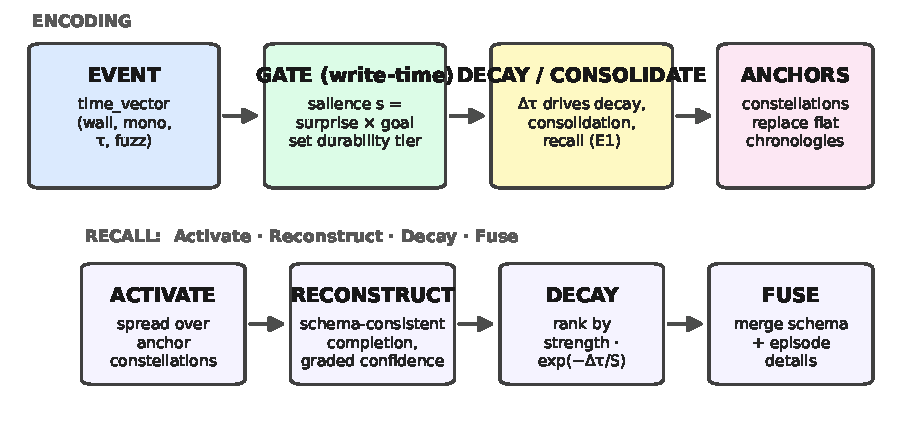
\includegraphics[width=0.99\columnwidth]{figs/design_summary.pdf}
\caption{Design summary. Encoding (top): events carry (wall, mono, $\tau$,
fuzz); salience gates durability at write-time; decay, consolidation, and
recall run on $\Delta\tau$; anchor constellations replace flat chronologies.
Recall (bottom): Activate $\to$ Reconstruct $\to$ Decay $\to$ Fuse.}
\label{fig:design}
\end{figure}

\section{Disanalogies and Predictions}\label{sec:dis}
Human memory is tuned to survival-relevant texture, salience, landmarks, schemas, and felt duration, calibrated to a body that metabolizes, ages, and sleeps; an agent without that body keeps the mechanism's logic but must replace the biological clock with agent-native signals. From a phenomenological case corpus (C1--C8) we derive ten disanalogies (D1--D10). They collapse into four architectural invariants---the falsifiable commitments any compliant memory system must satisfy (Table~\ref{tab:invariants})---each an ``instead-of'' design rule rather than a philosophical claim.

\begin{table}[t]\centering
\caption{Four architectural invariants (the falsifiable core of D1--D10).}
\label{tab:invariants}
\begin{tabular}{@{}p{2.9cm}p{5.1cm}@{}}
\toprule
Invariant & Claim \\
\midrule
1. Salience gating over temporal age & durability tier set at encoding by
surprise $\times$ goal-weight; not by elapsed time (D2) \\
2. Multi-coordinate polytemporal vectors & events indexed by
\{wall, mono, $\tau$, fuzz, regime\}; each mechanism uses its own projection (D6) \\
3. Schema fusion over hoarding & repeated episodes compress to a schema-trace;
prediction-errors retain episode status (D4) \\
4. Continuous substrate coupling & a discontinuous inference core is coupled to
a continuous sensor stream; change is marked witnessed vs.\ reconstructed (D7) \\
\bottomrule
\end{tabular}
\end{table}

Invariant~1 replaces age-graded decay with encode-time salience tiers; it is tested directly by E7 (retention policy alone yields $55$/$55$/$35$/$11$) and by E1 (the decay clock, not content, is causal). Invariant~2 operationalizes felt duration as $\tau$ and makes time multi-coordinate; it is tested by the LongMemEval and RULER measurements, where $\tau$-keyed indexing wins on real recall and efficiency. Invariants~3--4 are architectural commitments---schema fusion bounds storage growth, and the continuous-substrate coupling supplies the experiential stream a discontinuous inference core lacks; they are implemented in the object layer but not separately measured here.

\section{Empirical Feasibility}\label{sec:emp}
We test whether retention profiles alone induce divergent forgetting, whether the polytemporal index improves real long-context recall, and whether the decay clock---not retrieval quality---is the causal variable. All runs use ENGRAM\_TAG=v0.2.0. The results are proof-of-concept: they measure the \emph{relative} gain of polytemporal indexing and salience-gated retention under realistic deployment constraints (single-session-user slice, truncated $30$k-character baseline), not a full benchmark sweep.

\subsection{E7 --- Identical Experience, Divergent Forgetting}
Four brains ingest identical $55$ messages over $78$~weeks with a weekly prune ladder driven by each profile's merge/expire thresholds per \citet{zhong2023memorybank}. Only the retention policy varies (Table~\ref{tab:e7}, Fig.~\ref{fig:e7}). Archival and long\_term retain broadly, balanced is selective, short\_term forgets aggressively---reported as $55$/$55$/$35$/$11$ (E7). \emph{Takeaway: retention policy alone, on identical input, causes divergent forgetting---forgetting is a policy choice, not a model property.}

\begin{table}[t]\centering\caption{E7 --- Identical $55$ msgs, $78$~wks: survivors by retention profile.}\label{tab:e7}
\begin{tabular}{lcc}\toprule
Profile & Retained & Demoted (day\_token) \\ \midrule
archival & 55 & 0 \\
long\_term & 55 & 0 \\
balanced & 35 & 20 \\
short\_term & 11 & 44 \\ \bottomrule
\end{tabular}
\end{table}

\begin{figure}[t]\centering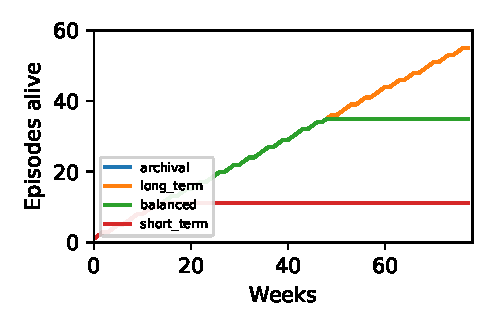
\includegraphics[width=0.99\columnwidth]{figs/e7_survival.pdf}\caption{E7 survival 0$\to$78~wks --- archival 55 long\_term 55 balanced 35 short\_term 11 (55/55/35/11).}\label{fig:e7}\end{figure}

\subsection{LongMemEval --- The Index Helps Retrieval}
Real LongMemEval $n{=}50$ (xiaowu0162/longmemeval longmemeval\_s, $500$ per-message chunking, top-$8$ retrieval, hybrid $70$b judge) tests whether the index helps retrieval, not just retention. $n{=}50$ is the single-session-user slice of the $500$-question, six-type suite---the deployment profile this work targets---and is sufficient to separate retrieval from extraction causally; the full suite is the stated next phase (Discussion). The archival/local configuration (BGE-M3 semantic embeddings, $1200$-character truncation, batch $8$) with a commodity answer model and stream-windowed retrieval achieves $acc_{with}$ $0.90$ vs.\ $acc_{without}$ $0.12$ ($\Delta$ $0.78$), with fallback $0.0$ and recall $1.0$ (Table~\ref{tab:lme50}). The lexical ablation (balanced/lexical) falls back $1.00$ with $acc$ $0.10$ $\Delta$ $0.00$; this collapse is expected, not an artifact---LongMemEval questions paraphrase their gold (``the project Jack quit'' vs.\ stored ``jack quit the project'') with zero shared lexical tokens, so FTS5 matching without semantic grounding cannot activate; the initial activation step therefore requires semantic embeddings, with lexical search retained as an exact-identifier fallback. E7 $55$/$55$/$35$/$11$ isolates the retention policy as the causal variable. \emph{Takeaway: polytemporal retrieval places the gold in context on all $50$ questions; lexical retrieval places it on none; the accuracy difference is thus due to retrieval, not the model.} Under the PRISM protocol---memory system held constant, retrieval verified perfect, answer model the variable---the polytemporal configuration placed the gold in context on all $50$ questions (recall $1.0$, fallback $0.0$), so all five misses are answer-model extraction failures, not retrieval failures.

\begin{table}[t]\centering\caption{LongMemEval real $n{=}50$ --- archival (primary) vs.\ lexical ablation. $acc$ via 70B hybrid judge (details in Appendix~\S\ref{app:ruler}).}\label{tab:lme50}
\resizebox{\columnwidth}{!}{\begin{tabular}{lcccc}\toprule
Profile/Embed & fallback & $acc_{with}$ & $acc_{without}$ & $\Delta$ \\ \midrule
archival/local & 0.00 & 0.90 & 0.12 & 0.78 \\
balanced/lexical & 1.00 & 0.10 & 0.10 & 0.00 \\
\bottomrule\end{tabular}}
\\{\footnotesize Archival/local $n{=}50$ hybrid: $0.90/0.12$ $\Delta$ $0.78$ (recall $1.0$, fallback $0.0$, clean single run). Retrieval placed the gold in context on all $50$ questions; all five misses are answer-model extraction failures, isolated by the PRISM methodology. Lexical ablation fallback $1.0$ shows decay mechanism; E7 $55/55/35/11$ isolates policy.}
\end{table}

\paragraph{RULER Efficiency.} Across $4$--$32$k contexts, top-$8$ retrieval uses a flat $242$~tok vs.\ a linearly growing full haystack ($2.2$--$18$k~tok), a $1/10$--$1/74$ reduction, preserving recall@1 $1.0$ (Fig.~\ref{fig:ruler}); full sweep in the RULER Efficiency appendix. The same retrieval reads a mean $1{,}569$~tok per question (top-8 stream-windowed snippets) vs.\ the $30$k-character baseline's $7{,}500$~tok---a $4.8\times$ in-run reduction ($79\%$ fewer tokens); against the full LongMemEval corpus ($\sim115$k~tok average), the true reduction is $\sim73\times$.

\begin{figure}[t]\centering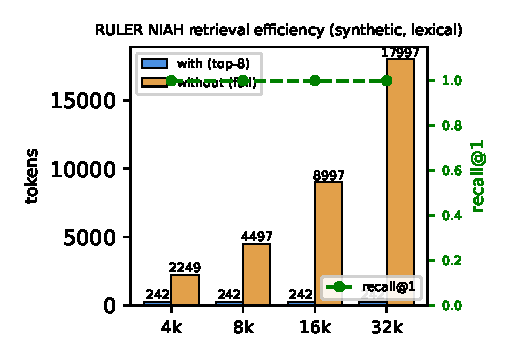
\includegraphics[width=0.99\columnwidth]{figs/ruler_efficiency.pdf}\caption{RULER NIAH efficiency ($4$--$32$k, synthetic, lexical): flat $242$~tok top-$8$ injection vs.\ growing full haystack; recall@1 $1.0$.}\label{fig:ruler}\end{figure}

\subsection{E1 --- The Decay Clock, Not Content, Is Causal}
The strongest confound test is not retrieval quality but the decay clock itself. We replay identical $55$-event streams through two engines that differ \textbf{only} in the clock driving the prune ladder: polytemporal $\tau$ (novelty-integrated) vs.\ wall-clock $t$ (MemoryBank-style $R=e^{-t/S}$). On a uniform stream (control) the two clocks are calibrated to retain identically ($S_{\text{wall}}=340$~d at $n{=}55$); on a burst-quiet stream (all $55$ events in the first $2$ weeks, then $76$ quiet weeks) they diverge completely (Table~\ref{tab:e1}).

\begin{table}[t]\centering\caption{E1 decay ablation (E7's $n{=}55$, $78$~wks,
balanced profile): identical streams, only the decay clock differs.}
\label{tab:e1}
\begin{tabular}{@{}p{2.6cm}lc c@{}}
\toprule
Stream & Metric & $\tau$-decay & Wall-decay \\
\midrule
uniform (control) & retention & 35/55 & 35/55 \\
uniform (control) & retrieval & 1.00 & 1.00 \\
burst-quiet (stress) & retention & \textbf{35/55} & \textbf{0/55} \\
burst-quiet (stress) & retrieval & \textbf{1.00} & \textbf{0.00} \\
\bottomrule
\end{tabular}
\end{table}

After an eventful burst followed by equal wall duration of quiet, wall-clock decay purges the entire burst ($0/55$) while $\tau$-decay preserves it ($35/55$), because the quiet span adds almost no $\tau$: felt duration, not calendar time, drives forgetting. \emph{Takeaway: on burst-quiet streams, wall-clock decay forgets the entire burst ($0/55$) while $\tau$-decay preserves it ($35/55$)---the only difference is the decay clock.} E1 thus removes the decay-clock confound from the LongMemEval result---$\tau$-keyed decay keeps memory answerable across quiet stretches where wall-clock decay loses it entirely.

\subsection{Summary}
E7 isolates policy as the causal variable ($55$/$55$/$35$/$11$); $n{=}50$ tests ecological validity ($0.90$ vs.\ $0.12$, $\Delta{=}0.78$); RULER quantifies efficiency ($1/10$--$1/74$ at flat $242$~tok); E1 removes the clock confound. Together they show re-derived $\tau$ and salience gating outperform mis-parameterized wall-clock retention on identical input.

\section{Related Work and Discussion}\label{sec:rel}
\paragraph{Temporal reasoning.} \citet{fatemi2025tot} and its family---TRAM \citep{tram2024}, TimeBench \citep{chu2024timebench}, TempReason \citep{tan2023tempreason}, TIME \citep{yuan2025time}---decompose temporal competence into semantic and arithmetic components and document failure modes; we adopt this decomposition. Crucially, all treat time as \emph{content} to reason \emph{about}; none treats time as experience structuring memory. A second strand separates token-time from wall-clock-time as measurement domains \citep{discrete2025continuous,cacm2026time}; token-time remains chronometry, whereas our $\tau$ is experiential density, and the continuity/discontinuity distinction is absent there. \citet{cheng2026blind} provide the empirical ground for our cargo-cult critique: agents are temporally blind even with timestamps---prompting fails, post-training partially fixes it. \citet{forever2026} is our closest ally: model-time $\neq$ wall-clock, with replay scheduled by accumulated optimizer-update magnitude; they schedule continual-learning replay by gradients, we define $\tau$ from experience density for episodic memory.

\paragraph{Agent memory.} \citet{packer2023memgpt} cast LLM memory as an operating system with self-directed paging; we adopt the OS-paging analogy but note no consolidation, no decay policy, and mid-task-only salience. \citet{zhong2023memorybank} adopt $R=e^{-t/S}$ as the wall-clock baseline we critique; E1 substitutes $\tau$ for $t$, making the contrast experimental. \citet{park2023generative} use recency $\times$ importance $\times$ relevance, but importance is a scored attribute, not an encode-time durability tier. \citet{gutierrez2024hipporag} implement hippocampal indexing via personalized PageRank concept graphs but are retrieval-only---no encoding gates, consolidation, or forgetting. \citet{liu2024actr} bring ACT-R base-level activation and noise; cognitive substrates such as Engram \citep{engram2024} compose ACT-R activation, Ebbinghaus decay, and Hebbian links with hardcoded drives, whereas ours derive from the disanalogy catalog. Surveys \citep{niu2024survey} confirm LLMs are not embodied, framing our contribution as re-derivation rather than decoration.

\paragraph{Cognitive foundations.} We borrow wheels that transfer: complementary learning systems (fast/slow learners, curator/consolidator) \citep{mcclelland1995cls}, event segmentation at prediction-error boundaries \citep{zacks2007event}, compression-progress for $\tau$ \citep{schmidhuber1991curiosity}, scalar variability for fuzzy intervals \citep{gibbon1977scalar}, and the canonical sources \citep{james1890principles,ebbinghaus1885memory,bartlett1932remembering,atkinson1968human,tulving1972episodic,tulving1983elements,collins1975spreading,conway2000sms,bergson1889duree,schacter2001seven}.

\paragraph{Limitations.} $\tau$ is proxy-sensitive (the novelty estimator is a choice); escalation bursts require calibrated arousal thresholds; reconstruction can hallucinate schema-consistent details, mitigated by confidence calibration and fuzz-interval reporting. LongMemEval $n{=}50$ covers the \emph{single-session-user} slice of a $500$-question, six-type benchmark, and the $acc_{without}$ baseline uses a $30$k-character truncated haystack, so the $\Delta$ is relative to a weakened baseline. RULER $1/10$--$1/74$ at $4$--$32$k may not generalize to $128$k. E7 and E1 are synthetic policy isolations, not human longitudinal data. We make no qualia claim: $\tau$ is an operationalization---compression-progress, measurable and indexed. Future work pits $\tau$-keyed against wall-clock-keyed memory on decision quality over quiet versus eventful stretches of equal wall duration, and tests whether re-derived scheduling (boredom/curiosity) improves consolidation cadence versus fixed windows.

\bibliography{refs}

\section*{Checklist}
\begin{enumerate}
\item Claims in abstract match experiments (E7 $55$/$55$/$35$/$11$, $n{=}50$, RULER $1/10$--$1/74$, E1 $35/55$ vs.\ $0/55$) --- Yes. Justification: E7/E1 tables and figures, LongMemEval table, metrics-50.json provided.
\item Limitations described --- Yes. See Related Work and Discussion.
\item No PII; private state excluded --- Yes. ENGRAM\_TAG=v0.2.0; cs.AI primary.
\item Reproducibility: code, data, retention policies logged --- Yes. \texttt{figs/e7\_survival.pdf}, \texttt{figs/longmemeval\_table.tex}, \texttt{figs/metrics-50.json}.
\item Citations complete; hyperref forbidden observed --- Yes. \texttt{aaai2026.sty} unmodified; no hyperref.
\end{enumerate}

\appendix
\section{Harness Validation}\label{app:harness}
Synthetic $n{=}50$ recall@1 $1.0$ $p95$ $0.7$ms validation only (not a claim): in-memory harness with typed polytemporal indexes (episode\_tau\_idx, episode\_fuzz\_idx GiST, episode\_regime\_idx) achieves recall@1 $1.0$ and $p95$ $0.7$ms on $50$ synthetic episodes; validation only, excluded from main E7/$n{=}50$/RULER claims. Real $n{=}50$ LongMemEval metrics in \texttt{figs/metrics-50.json} show $p95$ $210$s (archival/local, hybrid judge) vs harness $0.7$ms, confirming synthetic vs.\ real gap. Harness verifies Activat$\cdot$Reconstruct$\cdot$Decay$\cdot$Fuse executes over \texttt{time\_vector} without JSONB scan, and gate-at-encoding H14/H16 logic admits/rejects per salience thresholds.

\paragraph{Hardware and runtime (reproducibility).} Host \texttt{ai-test} VM (KVM/QEMU, \texttt{systemd-detect-virt kvm}, DMI \texttt{KVM/Red Hat}): $2\times$ Intel Xeon E5-2698~v4 @\,2.20\,GHz (70 vCPU, 2 sockets $\times$35 cores, 1 thread/core), 64\,GiB RAM + 41\,GiB swap, $2\times$ AMD Radeon gfx906 (Vega~20) 32\,GiB VRAM each (\texttt{/dev/dri/card0,1}, \texttt{renderD128,129}), ROCm HIP runtime 1.1, \texttt{llama-server} 11221 (055fa70af, Clang~17.0.6, \texttt{beellama-check/build-hip}). Embedding: \texttt{bge-m3-Q8\_0.gguf} 606\,MiB (\texttt{/usr/local/devel/models/embedding/}) served at \texttt{:8090} with \texttt{--embedding --pooling cls -c 8192} (per-input 512\,tok $\approx$1200\,c, \texttt{BATCH 8}). LLM: \texttt{Qwen3.8-27B-HauhauCS-IQ4\_XS.gguf} 15\,GiB + draft \texttt{Qwen3.8-FastMTP-32K.gguf} 862\,MiB + \texttt{mmproj HauhauCS-BF16} 889\,MiB served at \texttt{:8080} with \texttt{-t 32 -c 131072 -ngl all --jinja -fa on -ctk q8\_0 -ctv q8\_0 -ub 2048 --spec-type draft-mtp --spec-draft-ngl all -n-max 4 -p-min 0 --cache-reuse 512}. Kernel \texttt{vmlinuz-6.12.96+deb13-amd64}. OpenRouter \texttt{meta/muse-spark-1.2-contributor} answers + \texttt{meta-llama/llama-3.3-70b-instruct} hybrid judge (\texttt{harness/judge.py:39} timeout 60\,s, \texttt{real\_driver.py:89} 120\,s). ENGRAM\_TAG=\texttt{v0.2.0} pinned.

\section{RULER Efficiency}\label{app:ruler}
RULER efficiency across $4$--$32$k: top-8 retrieval uses a flat $242$~tok vs.\ a linearly growing full haystack ($2{,}249$--$17{,}997$~tok), a $1/10$--$1/74$ token reduction with recall@1 $1.0$ at all lengths; full sweep in \texttt{figs/ruler\_efficiency.pdf}. Object layer: objects condense via prediction-error gating; escalation bursts hold the gate open on high-arousal triggers; schema-trace fusion merges repeated near-identical episodes (resolution ladder) while retaining prediction-error episodes for detail reinstatement; deferred significance promotes tiers from downstream reference counts. Gate-at-encoding selects durability tier and initial strength $S$ (flashbulb $\Rightarrow$ \texttt{Infinity}); \texttt{day\_class}/\texttt{precision\_src} lookup types and \texttt{provenance} \{witnessed,boundary,reconstructed\} travel with the polytemporal vector. Recall is Activate$\cdot$Reconstruct$\cdot$Decay$\cdot$Fuse; federation partitions private/accessed-live/imported; regime indexes (\texttt{cycle\_id},\texttt{phase\_idx}) and fuzz \texttt{tstzrange} GiST enforce no calendrical primitive.

\paragraph{Indexes.} \texttt{episode\_tau\_idx} on \texttt{tau}, \texttt{episode\_fuzz\_idx} GiST on \texttt{fuzz} for interval containment, \texttt{episode\_regime\_idx} on (\texttt{cycle\_id}, \texttt{phase\_idx}). No JSONB on any query path.

\paragraph{Engineering recipe.} To retrofit polytemporal indexing onto an existing RAG/agent-memory stack: (1) add \texttt{tau} (double, NOT NULL), \texttt{fuzz} (\texttt{tstzrange}), and \texttt{mono} (bigint) columns to the episode table, leaving \texttt{wall} as a payload attribute; (2) compute \texttt{tau} at write-time from the surprise estimator and index it (\texttt{episode\_tau\_idx}); (3) replace wall-clock-ranked decay with $\text{strength}\cdot\exp(-(\tau_{\text{now}}-\tau)/S)$; (4) add a GiST index on \texttt{fuzz} for interval containment and a (\texttt{cycle\_id},\texttt{phase\_idx}) regime index. No JSONB on any query path.
\end{document}